\chapter{Steering}
The control of steering wheel take advantage of motor for steering assist originally present in the car. The motor is controlled by a positioning controllers designed for brushed DC and brushless DC motors with encoders. denominated \gls{EPOS} by many manufactures

\section{Maxon EPOS 70/10 controller}
\begin{figure}[h]
	\centering
	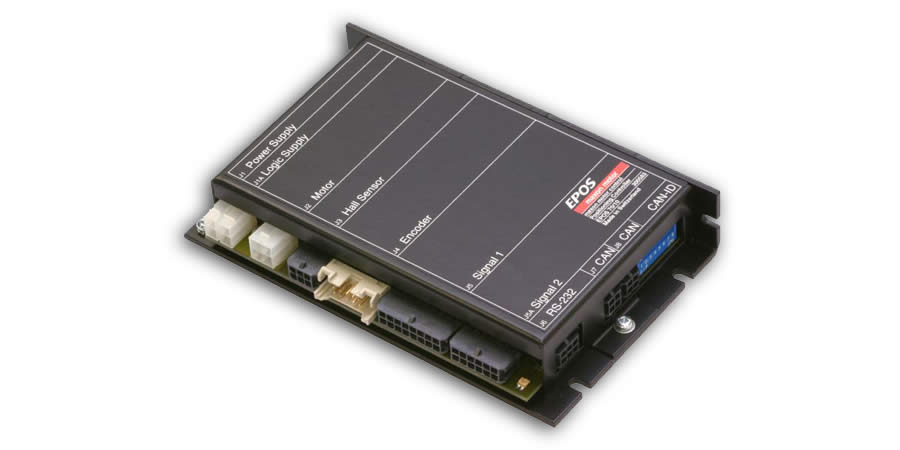
\includegraphics[width=0.5\linewidth]{figures/EPOS-70-10-10-A-11-70VDC-Detail.jpg}
	\caption{Maxon EPOS 70/10 controller}
	\label{fig:maxon_epos}
\end{figure}
The controller available to use is the \href{https://www.maxonmotor.com/maxon/view/product/control/Positionierung/300583}{Maxon EPOS 70/10}, from now on denoted as EPOS. It includes CAN network interface and a RS-232. The relevant electrical specs can be seen in table \ref{tab:epos_specs}. The full specifications as well as connections layout must be seen in \cite{epos_hardware}. The controller contains two led in a single package that is used as status reference. Table \ref{tab:maxon_led_status} present the status of device based on pattern of leds shown by it.
The \gls{EPOS} will be used as a \gls{PID} controller for the steering wheel.

\begin{table}[hb]
	\centering
	\begin{tabular}{lccc}
		\toprule
		\textbf{Description} & \textbf{Min.} & \textbf{Max.} & \textbf{Unity}\\
		\midrule
		Power supply voltage $\text{V}_\text{CC}$ (Ripple \textless 10\%) & 11 & 70 & $\text{V}_\text{DC}$\\
		Max. output voltage & & $0.9\cdot\text{V}_\text{CC}$ & $\text{V}_\text{DC}$\\
		Max. output current $\text{I}_\text{max}$ (\textless 1sec) &  & 25 & A\\
		Continuous output current $\text{I}_\text{cont}$ & & 10 & A\\
		Sample rate PI - current controller &10K & 10K & Hz\\ 
		Sample rate PI - speed controller  &1K & 1K & Hz\\ 
		Sample rate PI - positioning controller &1K & 1K & Hz\\
		Max. speed (motors with 2 poles) & & 25K & rpm\\
		\bottomrule
	\end{tabular}
    \caption{EPOS electric specifications}
    \label{tab:epos_specs}
\end{table}

\begin{table}[!hb]
	\centering
	\begin{tabular}{p{0.7\textwidth}cc}
		\toprule
		\textbf{Description} & \textbf{Red} & \textbf{Green}\\
		\midrule
		\begin{minipage}{0.4\linewidth}
			The EPOS is in state:
			\begin{itemize}
				\item Switch ON Disabled
				\item Ready to Switch ON
				\item Switched ON
				\item The power stage is disabled
			\end{itemize} 
		\end{minipage} & OFF & Blinking ($\approx$ 1Hz)\\
	    \midrule
	    \begin{minipage}{0.5\linewidth}
	    	The EPOS is in state:
	    	\begin{itemize}
	    		\item Operation Enable
	    		\item Quick Stop Active
	    		\item The power stage is enabled
	    	\end{itemize} 
	    \end{minipage} & OFF & ON\\
        \midrule
        EPOS is in Fault State & ON & OFF\\
        \midrule
        EPOS is in temporary state Fault Reaction Active & ON & ON\\
        \midrule
        There is no valid firmware on the EPOS (due to a failed firmware download) & ON & Flashing \\ 
		\bottomrule
	\end{tabular}
	\caption{Maxon EPOS 70/10 Led status}
	\label{tab:maxon_led_status}
\end{table}


\section{Steering sensor support}
Maxon EPOS 70/10 accepts quadrature sensors to give feedback of position. The used sensor is a quadrature line driver with index (although index is disabled because its track is damaged). The sensor model is HEDR-55L2-BY09 with main characteristics shown in table \ref{tab:quad_sensor} \cite{hedr_sensor}. Table \ref{tab:quad_sensor_settings} show the required configuration to be passed to EPOS device to correctly use the steering controller. See appendix \ref{appendix:maxon} for further description.
\begin{table}[!hb]
	\centering
	\begin{tabular}{lc}
		\toprule
		\textbf{Description} & \textbf{Value}\\
		\midrule
		Line Driver & Yes\\
		Counts per revolution & 3600\\
		Total number of positions & 14400\\
		Shaft diameter & 8mm\\
		\bottomrule
	\end{tabular}
	\caption{Main HEDR-55L2\_BY09 sensor characteristics}
	\label{tab:quad_sensor}
\end{table}

\begin{table}[!hb]
	\centering
	\begin{tabular}{lc}
		\toprule
		\textbf{Description} & \textbf{Value}\\
		\midrule
		Sensor Type & 2\\
		Pulse Number & 3600\\
		Sensor Polarity & 0\\
		\bottomrule
	\end{tabular}
	\caption{Quadrature sensor settings configured in EPOS}
	\label{tab:quad_sensor_settings}
\end{table}

The sensor support is mainly 3D printed in ABS filament. It is composed of the following parts presented in table \ref{tab:sensor_support_parts}.
A dimensional sketch of the sensor and bearing used was also designed just for auxiliary purposes and to provide assembly instructions. The drawings with respective dimensions are added in appendix \ref{appendix:sensor_drawings}. The parts were designed in Autodesk Fusion 360 and are available under the Github repository

\begin{table}[!hb]
    \centering
	\begin{tabular}{lcc}
		\toprule
		\textbf{Part name} & \textbf{Quantity} & \textbf{Reference design}\\
		\midrule
		608 bearing & 1 & \hyperref[draw:bearing]{Bearing Diagram}\\
		Sensor Case HEDR-55L2\_BY09 & 1 & \hyperref[draw:sensor-case]{Sensor case}\\
        Half Gear 54 teeth & 2 & \hyperref[draw:half-gear]{Half gear}\\
        Sensor gear 32 teeth & 1 & \hyperref[draw:sensor-gear]{Sensor gear}\\
		\bottomrule
	\end{tabular}
\caption{Sensor support parts}
\label{tab:sensor_support_parts}
\end{table}


\section{Calibration process}
Here is assumed the vehicle follows a model of Ackermann steering model typical valid for low speed which result in the simplified approximation of the single line model or as in general described in literature, as bicycle model\cite{Snider2009} \cite{Navigation_System_Design}. A simplified representation of the model is present in figure \ref{fig:ackermann_steering}. This model is normally used in control applications and expected to be used in future high level control. As it is necessary to determine the angle of wheel with respect to body frame YY axis (recall subsection \ref{subsection:body_frame}), the first calibration process required is to determine the function relating steering wheel position and angle of fictional wheel. A set up was made fixing the car and placing a white duck tape in front of it, perpendicular as physically possible and apart by 1.47 meters in front of the car. The duck tape will serve as a ruler. In each wheel is attached a laser level, pointing to front duck tape. Several measurements are take for different steering position values and using trigonometric relations, the angles of each wheel is estimated. 

The other calibration process is taken each time a power up is made. It consists in performing a full rotation of the steering wheel to each extreme points. During this movement, the program is always reading sensor position and updating the maximum and minimum value read. After these quadrature counter values are found, user is requested to end calibration and the offset are calculated and stored along with maximum and minimum position. These values will only change in case of shut down performed on steering controller device.

\begin{figure}[]
	\centering
	\subcaptionbox{Four wheel representation}{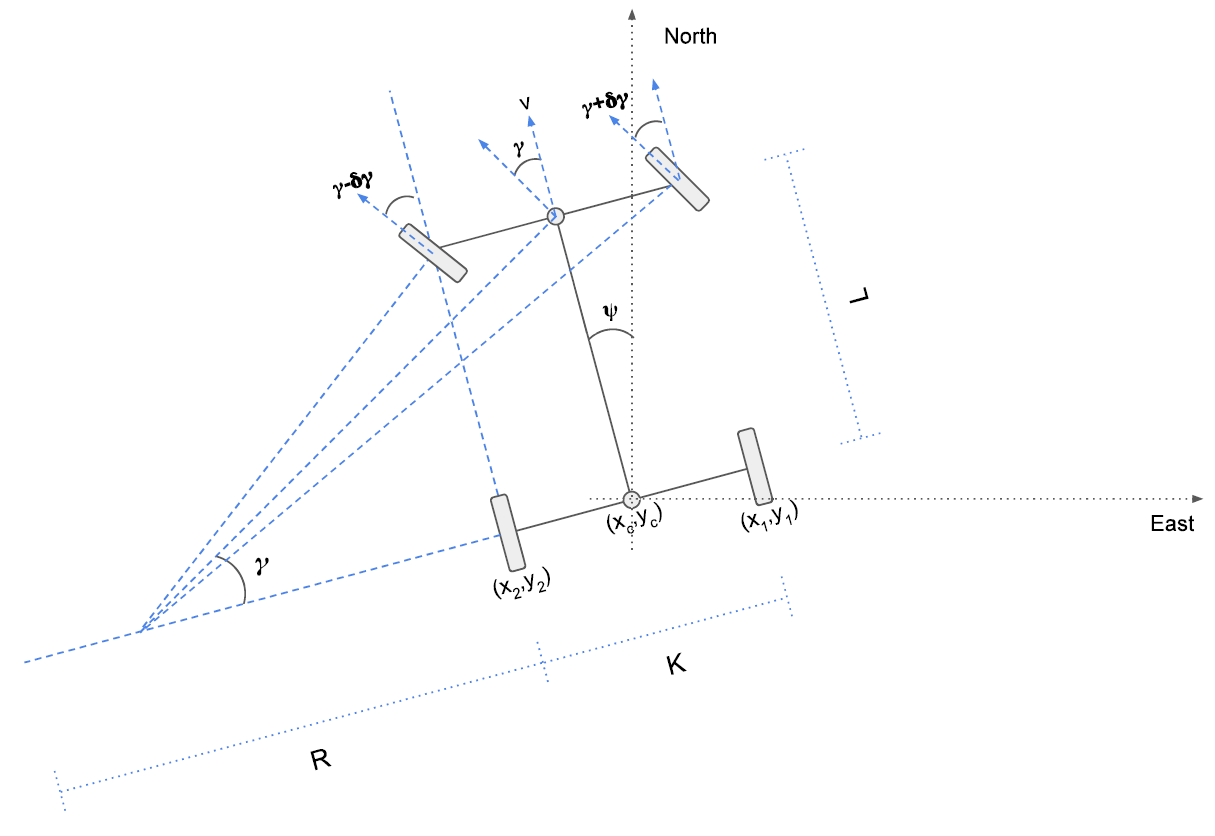
\includegraphics[width=0.7\linewidth]{figures/Ackermann_steering.png}}
	\hfill
	\subcaptionbox{Bicycle Representation (source \cite{Snider2009})}{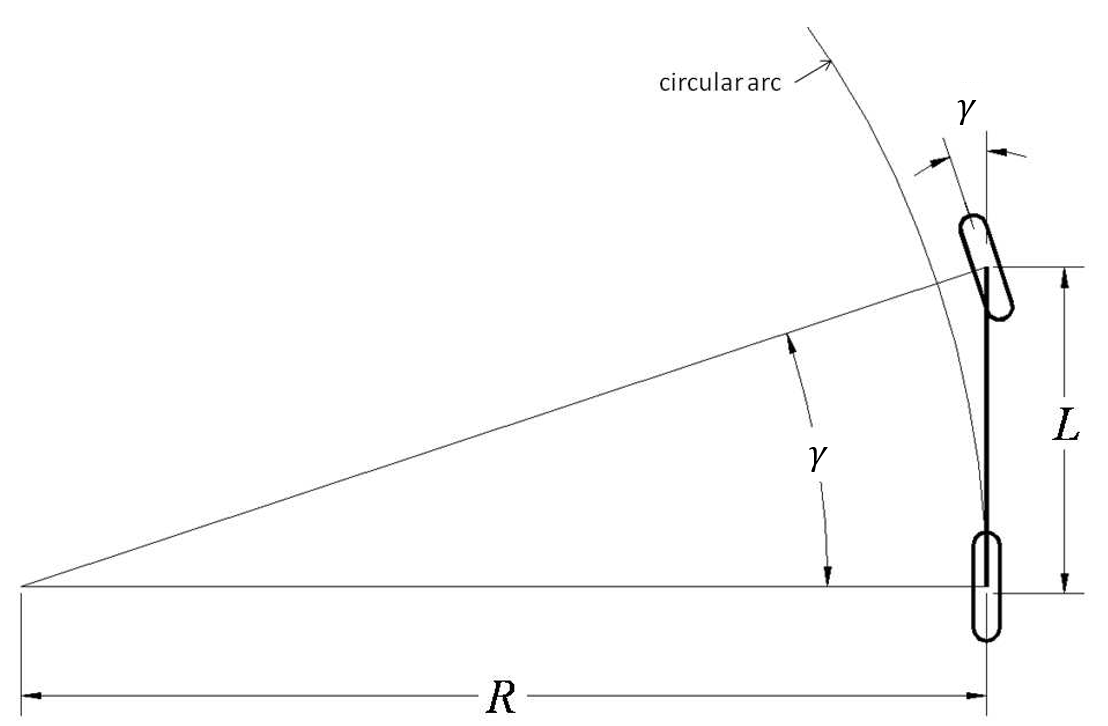
\includegraphics[width=0.5\linewidth]{figures/bicycle_model}}
	\caption{Ackermann steering model simplification}
	\label{fig:ackermann_steering}
\end{figure}

Taking figure \ref{fig:calibration_scheme} that represents the calibration set up made, the bold line between points $max_L$ and $max_R$ represent the our ruler. The $d1$ represent the distance between outer of each wheel where the lasers are attached. The relevant distances using in this step up are present in table \ref{tab:calibration_scheme}.
\begin{figure}[!h]
	\centering
	\begin{tikzpicture}[scale=2.5]
	\pgfmathsetmacro{\hOne}{1.47};
	\pgfmathsetmacro{\dOne}{1.445};
	\pgfmathsetmacro{\dL}{0.455};
	\pgfmathsetmacro{\maxR}{2.19};
	\pgfmathsetmacro{\maxL}{\maxR};
	\pgfmathsetmacro{\maxRange}{\maxR+\maxL+\dL};
	\pgfmathsetmacro{\lOne}{0.5*(\maxRange-\dL)};
	\pgfmathsetmacro{\lTwo}{0.5*(\dOne-\dL)};
	
	\coordinate (origin) at (0, 0);
	\coordinate (A) at (-\dOne/2, 0);
	\coordinate (B) at (\dOne/2, 0);
	\coordinate (C) at (-\dOne/2, \hOne);
	\coordinate (D) at (\dOne/2, \hOne);
	\coordinate (E) at (-\dOne/2 - \lOne, \hOne);
	\coordinate (F) at (\dOne/2 + \lOne, \hOne);
	\coordinate (zeroR) at (-\dL/2,\hOne);
	\coordinate (zeroL) at (+\dL/2,\hOne);
	
	
	\draw [Bar-Bar , ultra thick] (A)--(0,0) -- (B) node[align=center, below] at (origin) {$d_1$};
	\draw [dashed] (A) -- (C) node[below, midway, rotate=90] {$h_1$};
	\draw [dashed] (B) -- (D);
	\draw [dashed] (origin) -- ++(0, 6mm);
	\draw [Bar-Bar,ultra thick] (E)--(F);
	% add angles swipes lines
	\draw [dashed] (A)--(E);
	\draw [dashed] (A)--(zeroL);
	\draw [dashed] (B)--(F);
	\draw [dashed] (B)--(zeroR);
	
	% add zeroR and zeroL nodes
	\node[mark=square, fill, label=above:$0_R$] at (zeroR) {};
	\node[mark=square, fill, label=above:$0_L$] at (zeroL) {};
	% add maxR and maxL nodes
	\node[label=above:$max_R$] at (F) {};
	\node[label=above:$max_L$] at (E) {};
	
	% add arcs of angles
	\filldraw[fill=green!20,draw=green!50!black, dashed] (0,0) -- (0mm,5mm) arc (90:45+90:5mm) node[midway, above]{$\gamma$}-- (0,0);
	
	\filldraw[fill=cyan!20,draw=cyan!50!black, dashed] (A)--($(A)+(0mm,5mm)$) arc (90:56+90:5mm) node[midway, above]{$\beta$} -- (A);
	
	\filldraw[fill=red!20,draw=red!50!black, dashed] (B)--($(B)+(0mm,5mm)$) arc (90:33+90:5mm) node[midway, above]{$\alpha$}--(B);
	
	% add anotations
	\draw [Bar-Bar] (-\dOne/2,\hOne+0.3) -- (-\dL/2,\hOne+0.3) node[align=center, above, midway] {$L_2$};
	\draw [Bar-Bar] (-\dL/2,\hOne+0.3) -- (\dL/2,\hOne+0.3) node[align=center, above, midway] {$d_L$};
	\draw [Bar-Bar] (+\dL/2,\hOne+0.3) -- (\dOne/2,\hOne+0.3) node[align=center, above, midway] {$L_2$};
	\draw [Bar-Bar] (\dOne/2,\hOne+0.3) -- (\dOne/2 + \lOne, \hOne+0.3) node[align=center, above, midway] {$L_1$};
	\draw [Bar-Bar] (-\dOne/2,\hOne+0.3) -- (-\dOne/2 - \lOne, \hOne+0.3) node[align=center, above, midway] {$L_1$};
	\end{tikzpicture}
	\caption{Calibration set up scheme}
	\label{fig:calibration_scheme}
\end{figure}

\begin{table}[!hb]
	\centering
	\begin{tabular}{lc}
		\toprule
		\textbf{Description} & \textbf{Measurement [cm]}\\
		\midrule
		$d_1$ & 144.5\\
		$L_1$ & 124\\
		$L_2$ & 49.5\\
		$d_L$ & 45.5\\
		$h_1$ & 147\\
		$max_L$ & $L_1+L_2+d_L=$ 219\\
		$max_R$ & $L_1+L_2+d_L=$ 219\\
		\bottomrule
	\end{tabular}
	\caption{Reference measurements for calibration set up scheme}
	\label{tab:calibration_scheme}
\end{table}

Comparing figure \ref{fig:ackermann_steering} with figure \ref{fig:calibration_scheme} results in \eqref{eq:steeting_cal}. Then is assumed that:
\begin{itemize}
	\tightlist
	\item $\gamma$ must be a first order function.
	\item $\delta \gamma$ must be always great or equal to zero and therefore, quadratic.
	\item $\beta$ and $\alpha$ should be, at least a second order function with opposite concavities orientation.
\end{itemize}


\begin{equation}
\centering
\left \lbrace \begin{aligned}
\beta &= \gamma + \delta \gamma\\
\alpha&= \gamma - \delta \gamma
\end{aligned}
\right.
\label{eq:steeting_cal}
\end{equation}

Taking several measurements for different values of quadrature counters, is calculated the respective values of $\alpha$ and $\beta$. After, for each of those pairs is calculated the estimated values of $\delta \gamma$ and $\gamma$. Using least squares approach (\gls{polyfit} from Matlab\textregistered) is estimated the best fitting for each variable with respect to \gls{qc}, assuming the discussed points above. The result of fitting is shown in figure \ref{fig:calibration_results}. It shows the evaluated values of fitted functions in the range of -40000 to 40000 \gls{qc}. Note the fact that zero value is slightly apart to the right. This is a normal consequence of small misalignment (approximate 1\degree) of wheels when the \gls{EPOS} device is initialized, which is assumed the zero of it. This reflects the requirement to perform the full rotation to each side after device power up, to find the offset at origin.

The estimated ration between steering wheel \gls{qc} and the fictional wheel of bicycle model is then $-7.5014E-04$, translating in the equation \eqref{eq:qc_to_angle}, where the offset is determined at each power up calibration step. 

The Matlab\texttrademark used for calibration is present in appendix \ref{appendix:calibration_script}

\begin{figure}[!hb]
	\centering
	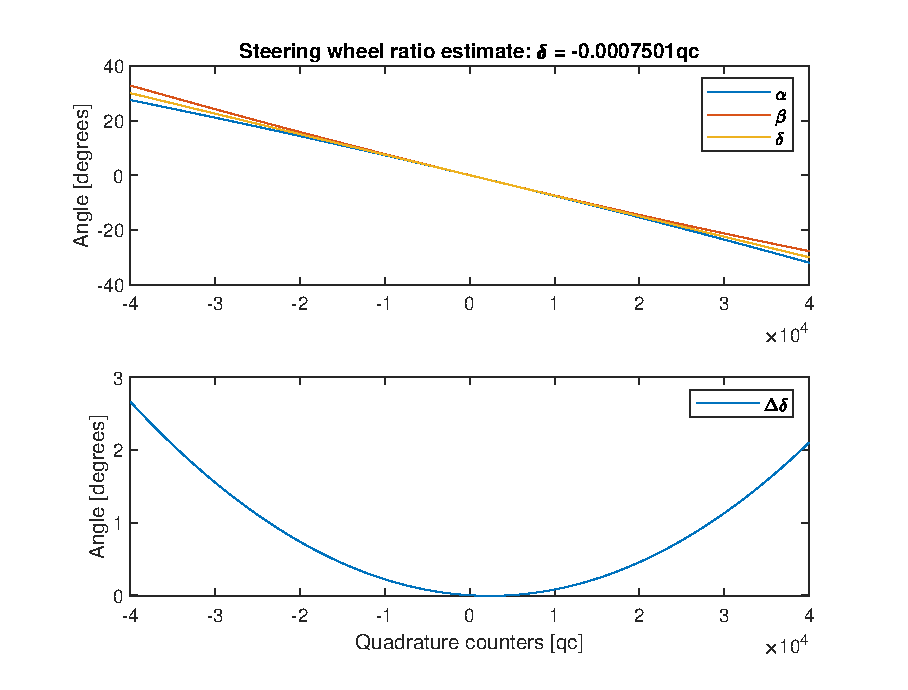
\includegraphics[width=0.7\linewidth]{figures/Steering_calibration_results.eps}
	\caption{Results for Calibration of steering wheel}
	\label{fig:calibration_results}
\end{figure}

\begin{equation}
f(qc) = -7.5014E-04 \times qc + offset
\label{eq:qc_to_angle}
\end{equation}


\section{interface library}

The developed interface library for \gls{EPOS} is present in the same Github repository. The library is made in python language and using the CAN interface to interact with \gls{EPOS}. User should note that the library still not cover all the possible interactions and modes of operation of \gls{EPOS}. It is only designed for position control mode. In the same repository are the firmware manual provided by Maxon and they should be consulted for further information. The respective documentation of the library is present on online version \href{https://maxon-epos-canopen.readthedocs.io/en/latest/}{here} and also as appendix \ref{appendix:maxon}. User should always prefer the online documentation to grant is the most updated version.


\section{Support and controller advices}
\begin{mdframed}[backgroundcolor=red!20, roundcorner=10pt]
	 Danger
\end{mdframed}
Since the sensor support is 3D printed, care must be taken to avoid abrupt variations of the steering wheel or the sensor gear might brake. User must also be careful to not apply achieve or surpass the extreme positions because it may cause damage to either the structure of car or the motor it self.

The \gls{EPOS} contains built-in function that disables the operation if difference between the demanded position and current position grows or is higher beyond the predefined maximum following error parameter. These situation can be caused by a badly conditioned reference, if the motor is blocked or if the motor is not able to keep up with the rate of variation requested. A careful reference trajectory generation must be provided by user to avoid damage. During the testing of vehicle in field and development, a series of functions have been developed that can serve as inspiration for future implementations. They are presented in appendix \ref{appendix:steering_auxiliar_class} in the form of a Python class.

 